%=========================Preamble====================================%
\documentclass[12pt] {article}
\usepackage{times}
\usepackage[margin=1in,bottom=1in,top=0.5in]{geometry}

\usepackage{graphicx}


\usepackage{float}
\usepackage{graphicx}
\usepackage{subfig}
\usepackage{wrapfig,lipsum}
\usepackage{amssymb}
\usepackage{nath}
\usepackage{amsfonts}


%=========================Doc====================================%
\begin{document}
\title{ECE 289A - An Introduction to Reinforcement Learning HW\#2}

\author{Ahmed H. Mahmoud}
\date{October, 26th 2017} 
\maketitle
\section*{Q.1}
The Bellman equation for $q_{*}$ for the recycling robot is:
\begin{equation}
q_{*}(h,w) = p(h|h,w)[r(h,w,h) + \gamma max_{a^\prime} q_{*}(h,a^\prime)] = r_{w} + \gamma max_{a^\prime} q_{*}(h,a^\prime)
\end{equation}
\vline
\begin{equation}
q_{*}(h,s) = p(h|h,s)[r(h,s,h) + \gamma max_{a^\prime} q_{*}(h,a^\prime)] + p(l|h,s)[r(h,s,l) + \gamma max_{a^\prime} q_{*}(l,a^\prime)]\\ = \alpha[r_{s} + \gamma max_{a^\prime} q_{*}(h,a^\prime)] + (1-\alpha) [r_{s} + \gamma max_{a^\prime} q_{*}(l,a^\prime)]
\end{equation}
\vline
\begin{equation}
q_{*}(l,w) = p(l|l,w)[r(l,w,l) + \gamma max_{a^\prime} q_{*}(l,a^\prime)]= r_{w} + \gamma max_{a^\prime} q_{*}(l,a^\prime)
\end{equation}
\vline
\begin{equation}
q_{*}(l,s) = p(l|l,s)[r(l,s,l) + \gamma max_{a^\prime} q_{*}(l,a^\prime)] + p(h|l,s)[r(l,s,h) + \gamma max_{a^\prime} q_{*}(h,a^\prime)] \\
= \beta [r_{s} + \gamma max_{a^\prime} q_{*}(l,a^\prime)] + (1-\beta) [-3 + \gamma max_{a^\prime} q_{*}(h,a^\prime)] 
\end{equation}
\vline
\begin{equation}
q_{*}(l,re) = p(h|l,re)[r(l,re,h) + \gamma max_{a^\prime} q_{*}(l,a^\prime)]= \gamma max_{a^\prime} q_{*}(l,a^\prime)
\end{equation}
where $l$ and $h$ are the low and high state, the actions \emph{search}, \emph{wait} and \emph{recharge} are given the abbreviated as $s$, $w$ and $re$. Also, $r_{s}$, $r_{w}$ are the expected number of cans to be collected while searching and waiting respectively i.e., the reward. We omitted all terms with zero probability. 

\section*{Q.2}
The following shows the optimal value function for Gridworld problem given in Example 3.12 by solving the Bellman equation for $v_{*}$.

\[
\begin{array}{|c|c|c|c|c|}
\hline
21.9775    & 24.4194     & 21.9775   & 19.4194  &  17.4775   \\
\hline
19.7797 &  21.9775 &  19.7797 &  17.8018 &  16.0216\\
\hline
17.8018  & 19.7797 &  17.8018 &  16.0216 &  14.4194\\
\hline
16.0216 &  17.8018 &  16.0216  & 14.4194  & 12.9775\\
\hline
14.4194  & 16.0216  & 14.4194 &  12.9775 &  11.6797\\
\hline
\end{array} 
\]



\section*{Q.3}
For this question, we started first by generating the original figures to the problem as descried in Example 4.2 to make sure the code works correctly before adding any additional conditions. Figure \ref{fig:original} shows the solution; the policy as it improves until we reach the optimal policy along with the optimal value function. These results are identical to the one given in the book (Figure 4.2 in the book).

\begin{figure}[!tbh]
\centering        
   \subfloat {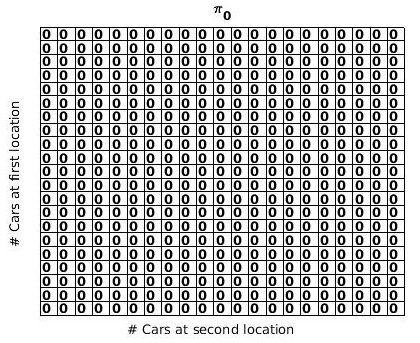
\includegraphics[width=0.35\textwidth]{../original_pi0.jpg}}
   \subfloat {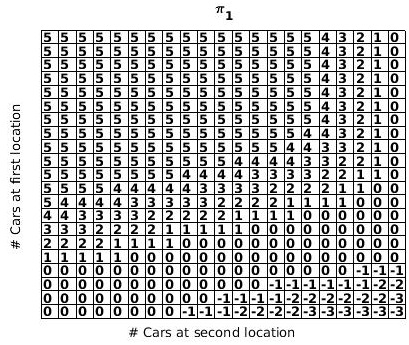
\includegraphics[width=0.35\textwidth]{../original_pi1.jpg}}
   \subfloat {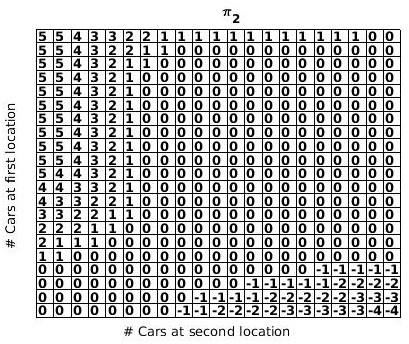
\includegraphics[width=0.35\textwidth]{../original_pi2.jpg}}
        
   \subfloat {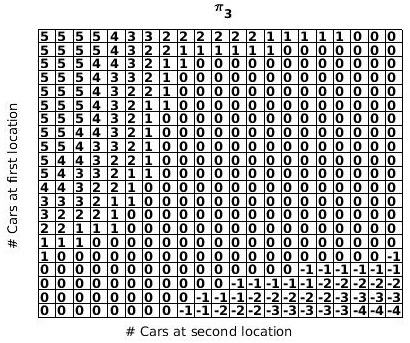
\includegraphics[width=0.35\textwidth]{../original_pi3.jpg}}
   \subfloat {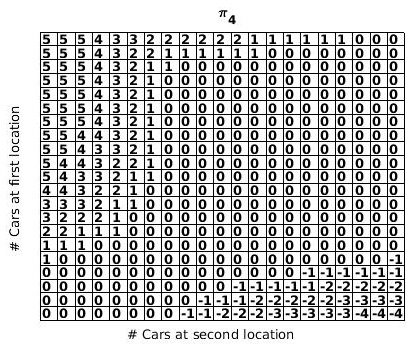
\includegraphics[width=0.35\textwidth]{../original_pi4.jpg}}
   \subfloat {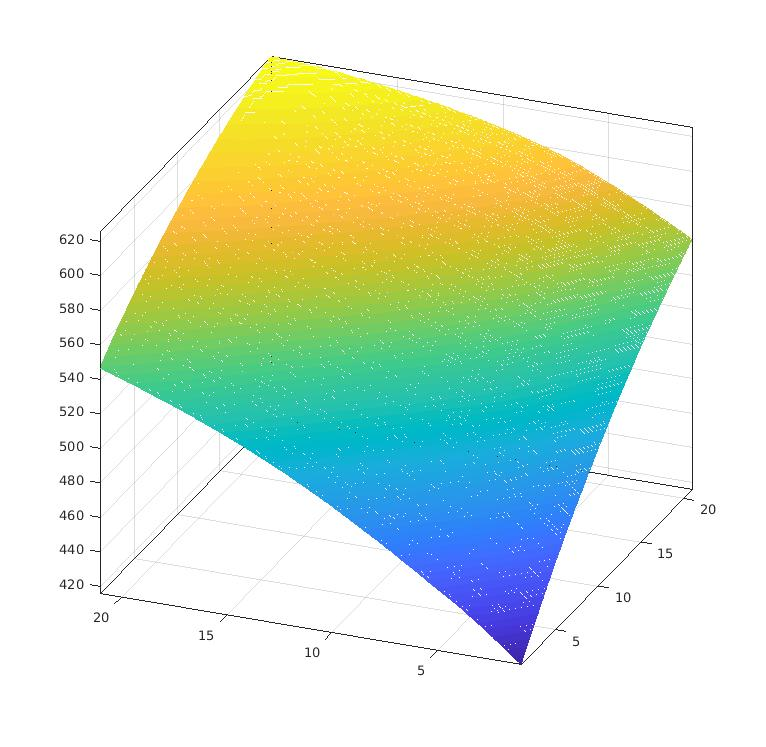
\includegraphics[width=0.35\textwidth]{../original_final_state_val_func.jpg}}     
   \caption{Regenerated original Jack's car rental as described in Example 4.2 without any additional conditions. }
   \label{fig:original}
\end{figure}

Next, we added the new conditions by incurring no cost for the first car moved from the first location to second location. Also, we decreased the reward by 4 whenever there are more than 10 cars in any location (strictly more than). Figure \ref{fig:bae} shows the improved policy and the optimal value function. 

\begin{figure}[!tbh]
\centering        
   \subfloat {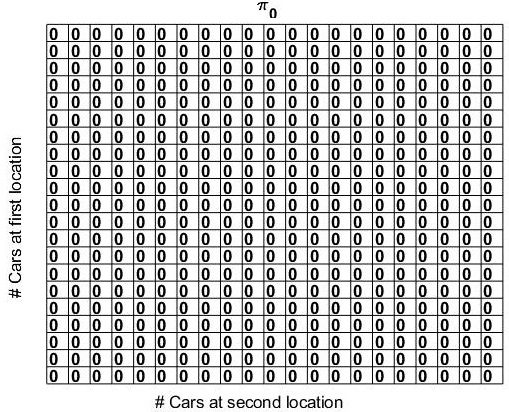
\includegraphics[width=0.35\textwidth]{../pi0.jpg}}
   \subfloat {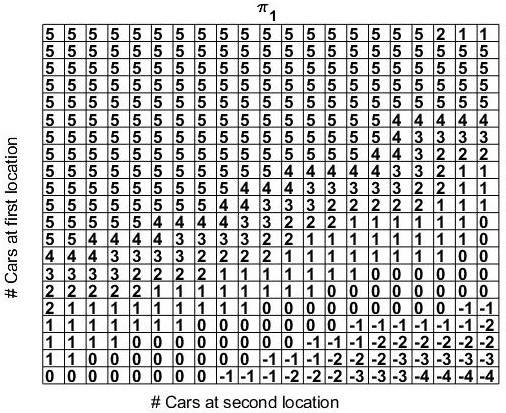
\includegraphics[width=0.35\textwidth]{../pi1.jpg}}
   \subfloat {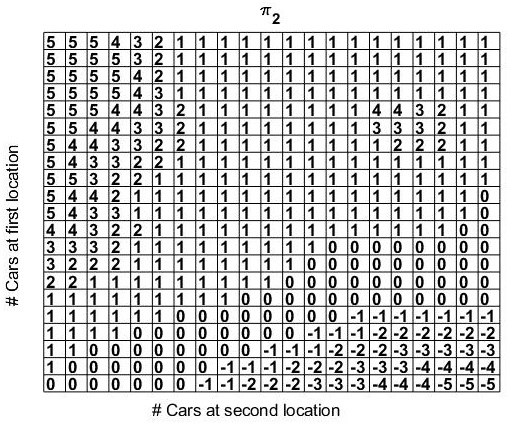
\includegraphics[width=0.35\textwidth]{../pi2.jpg}}
        
   \subfloat {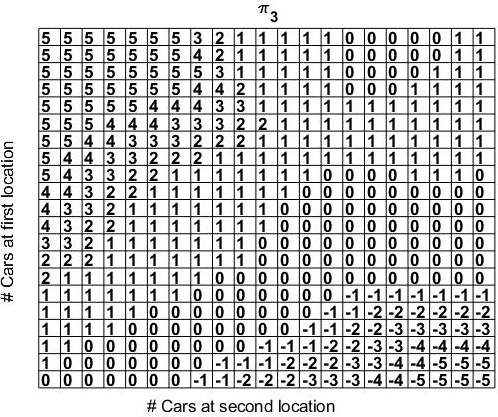
\includegraphics[width=0.35\textwidth]{../pi3.jpg}}
   \subfloat {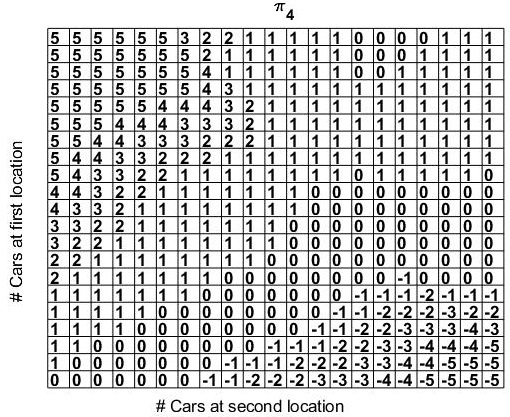
\includegraphics[width=0.35\textwidth]{../pi4.jpg}}
   \subfloat {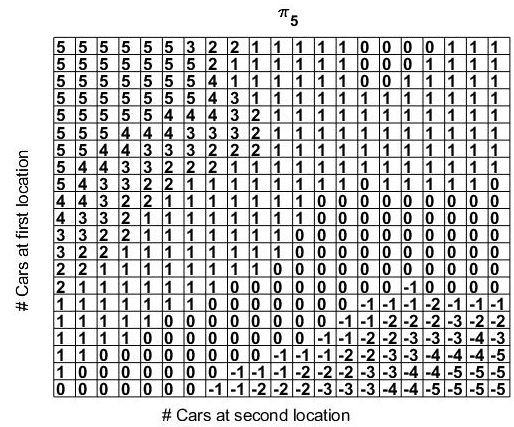
\includegraphics[width=0.35\textwidth]{../pi5.jpg}}
   
   \subfloat {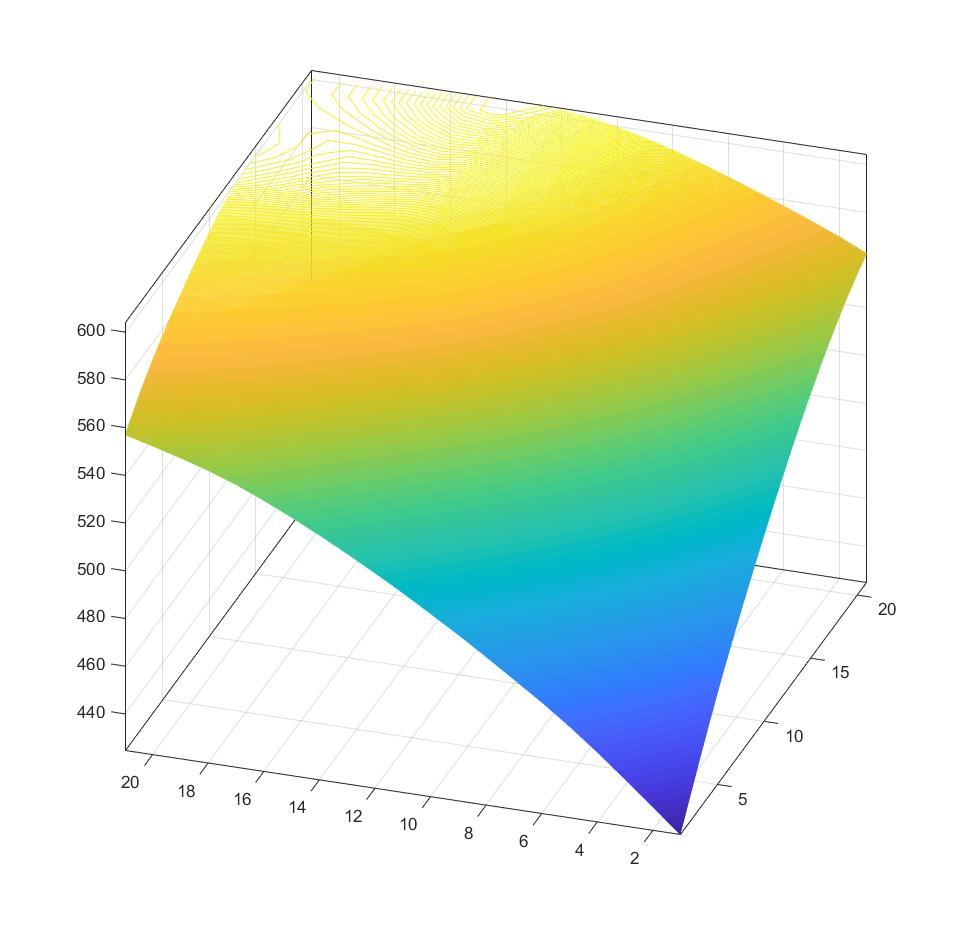
\includegraphics[width=0.45\textwidth]{../final_state_val_func.jpg}}     
   \caption{Solution for Jack's car rental after adding the new conditions as described in Exercise 4.4; the policy as it improves till we reach the optimal policy along with the optimal value function.}
   \label{fig:bae}
\end{figure}




\end{document}
